\subsection{Hierarchical Navigable Small World Graphs}\label{subsec:hierarchical-navigable-small-world-graphs}
A Hierarchical Navigable Small World graph (HNSW)~\cite{malkov_efficient_2020} is a data structure used to perform efficient information search with approximate K-Nearest Neighbors Search (K-NNS) algorithms.
The HNSW approach does not need any additional searching data structure.
The basic idea behind this approach is shown in Figure~\ref{fig:hnsw}.
A search will start at the highest layer (red dot) and then descend to the lower layers based on the result of the greedy algorithm implemented in the HNSW algorithm (red dashed lines).
This descent will continue until we reach the goal (green dot). \\ \\
In the context of our thesis, we are not dealing with an exact K-NNS\@.
Exact K-NNS (Section~\ref{subsec:k-nearest-neighbors})~\cite{navarro_searching_2002, tellez_singleton_2016} is feasible when dealing with a small number of data points.
Since it scales linearly with the number of data points, it becomes unfeasible when performing an exact search in a large database.
This is caused by what's known as the \("\)curse of dimensionality\("\). \\ \\
This issue can be overcome by using an approximate K-NNS algorithm~\cite{muja_scalable_2014, houle_rank-based_2015}.
In the case of approximate K-NNS, we \("\)[relax] the condition of the exact search by allowing a small number of errors.\("\)~\cite{malkov_efficient_2020}
Obviously, the search results will not be as exact as those returned by a K-NNS algorithm, but this is acceptable for applications such as an information retrieval system.
Especially in our case, since we also have a filtering system that can help with the retrieval of the most similar documents. \\ \\
This approximate K-NNS and HNSW algorithm has been implemented in Elasticsearch\footnote{https://www.elastic.co/guide/en/elasticsearch/reference/current/knn-search.html\#approximate-knn-limitations}.
The HNSW is used by Elasticsearch to index the dense vectors (document embeddings), while the approximate K-NNS algorithm is used to retrieve the $K$ most similar documents to the query vector.

\begin{figure}[!h]
    \begin{center}
        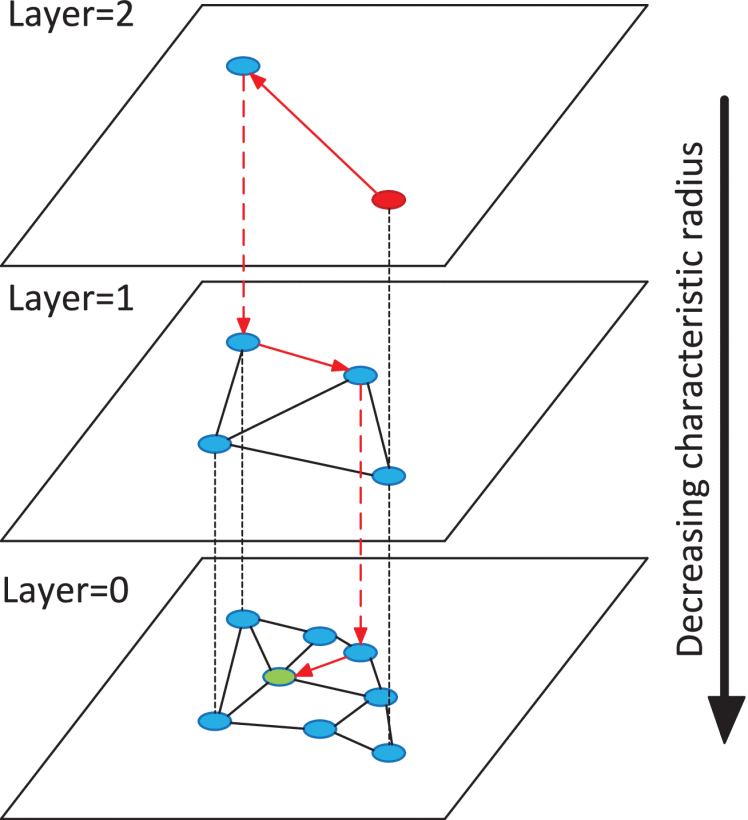
\includegraphics[width=0.3\linewidth]{assets/png/background/hnsw}
    \end{center}

    \caption{Idea behind the HNSW implementation~\cite{malkov_efficient_2020}}
    \label{fig:hnsw}
\end{figure}
